\section{Model}

A dataflow network can be modeled as the following matrix equation:

\begin{equation}
\textbf{P}=\textbf{U}\textbf{C}
\end{equation}

where \textbf{C} represents token consumption ports, \textbf{P} represents token production ports and \textbf{U} represents the utilisation of connections between producers and consumers. It can be re-written as:

\begin{equation}
\textbf{A}_{\textbf{p}}\textbf{P}=\textbf{U'}\textbf{A}_{\textbf{c}}\textbf{C}
\end{equation}

where \textbf{U'} represents the new utilisation of connections between producers and consumers, and $\textbf{A}_{\textbf{c}}$ and $\textbf{A}_{\textbf{p}}$ map consumer/producer ports to actors according to actor execution ratio (by default, identity matrix, i.e., all actors run during the entire time), respectively, such that:

\begin{equation}
\begin{pmatrix}
  a_{p1} & 0 & 0 & \cdots & 0 \\
  0 & a_{p2} & 0& \cdots & 0 \\
  0 & 0 & a_{p3} & \cdots & 0 \\
  \vdots  & \vdots  & \vdots & \ddots & \vdots  \\
  0 & 0 & 0& \cdots & a_{pm} 
 \end{pmatrix}
 \begin{pmatrix}
  p_{1}  \\
  p_{2}  \\
  p_{3}  \\
  \vdots  \\
  p_{m}  
 \end{pmatrix}
=
\begin{pmatrix}
  u_{1} & 0 & 0 & \cdots & 0 \\
  0 & u_{2} & 0& \cdots & 0 \\
  0 & 0 & u_{3} & \cdots & 0 \\
  \vdots  & \vdots  & \vdots & \ddots & \vdots  \\
  0 & 0 & 0& \cdots & u_{m} 
 \end{pmatrix}
\begin{pmatrix}
  a_{c1} & 0 & 0 & \cdots & 0 \\
  0 & a_{c2} & 0& \cdots & 0 \\
  0 & 0 & a_{c3} & \cdots & 0 \\
  \vdots  & \vdots  & \vdots & \ddots & \vdots  \\
  0 & 0 & 0& \cdots & a_{cm} 
 \end{pmatrix}
\begin{pmatrix}
  c_{1}  \\
  c_{2}  \\
  c_{3}  \\
  \vdots  \\
  c_{m}  
 \end{pmatrix}
\end{equation}


This can be re-written as the linear system:

\begin{equation}
 \begin{cases} 
 p_1 a_{p1}=u_1 a_{c1} c_1 \\
p_2 a_{p2}=u_2 a_{c2} c_2 \\
\vdots \\
p_m a_{pm}=u_m a_{cm} c_m
\end{cases}
\label{eq:solvable}
\end{equation}

Hence, the problem of scheduling a dynamic dataflow network, can be re-written as: \textit{choosing a \textbf{U'} diagonal matrix, such that the linear system in (\ref{eq:solvable}) is solvable, and such that the non-zero elements of \textbf{U'} are as close as possible to 1}. The last element in the definition can be formally described as:

\begin{equation}
min \sum_{n=1}^{m}{\sqrt{(u_{n,n}-1)^2}}
\end{equation} 

Two heuristics are important to simplify this analysis: 

\begin{equation}
\forall x: 0 < a_x \leq 1 \cap \forall n: 0 < u_{n,n} \leq 1
\end{equation} 


since actor execution ratio must be between 0 and 1, and queue utilization should have an upper limit of 1 to prevent full queues and corresponding deadlocks.


\subsection{Classification Matrices}

Having modeled a general dataflow network and specified the requirements for the existence of a solution (that the linear system in (\ref{eq:solvable}) is solvable) and formalised the problem within linear algebra, we can specify classification matrices (pairs of $\textbf{A}_{\textbf{c}}$ and $\textbf{A}_{\textbf{p}}$) which characterise particular dataflow network configurations, and analyse the problem for each classification.

\subsubsection{Single port feed forward}

Single port feed forward networks are the simplest type of dataflow networks. In this class, each actor has only one input and one output port: hence, the full network has one input and one output, resulting in the classification matrices:

\begin{equation}
\textbf{A}_{\textbf{p}}=
\begin{pmatrix}
   a_{1} & 0& \cdots & 0 \\
   0 & a_{2} & \cdots & 0 \\
   \vdots  & \vdots & \ddots & \vdots  \\
   0 & 0& \cdots & a_{m} 
 \end{pmatrix}
,
\textbf{A}_{\textbf{c}}=
\begin{pmatrix}
   a_{2} & 0& \cdots & 0 \\
   0 & a_{3} & \cdots & 0 \\
   \vdots  & \vdots & \ddots & \vdots  \\
   0 & 0& \cdots & 1 
 \end{pmatrix}
\end{equation} 

These matrices are characterised by having $\textbf{A}_{\textbf{p1,1}}=1$, $\textbf{A}_{\textbf{cm,m}}=1$ and no repeated actor mapping elements. Additionally, it is possible to name actors in such a way that actor mapping elements are ordered in both matrices (this is not possible in networks with feedback). The linear system solution for single port feed forward networks results in:

\begin{equation}
 \begin{cases} 
 p_1a_1=u_1c_1 a_2 \\
p_2 a_2=u_2 c_2 a_3 \\
\vdots \\
p_m a_m=u_m  c_m
\end{cases}
\label{eq:solvable}
\end{equation}

or, in augmented matrix form:

\begin{equation}
\begin{pmatrix}[cccc|c]
  p_1 & -u_1c_1 & 0 & \hdots & 0   \\
  0 & p_2 & -u_2c_2 & \hdots  &0  \\
  \vdots & \vdots &  \vdots & \ddots & \vdots \\
  0 & 0 & 0 & p_m & u_mc_m  
 \end{pmatrix}
\end{equation}

Since both the coefficient and augmented matrices have rank $m$ (the number of free variables), the system has a unique solution for any values of $\textbf{U'}$: hence, it is always possible to set all queue utilisations to 1 and determine actor execution ratios.
 

\subsubsection{Divergent feed forward}

In divergent feed forward networks, each actor has only one input port, but may have several output ports, resulting in networks that diverge into two or more independent paths: hence, the full network has one input and several outputs, resulting in the classification matrices:

\begin{equation}
\textbf{A}_{\textbf{p}}=
\begin{pmatrix}
   a_{\textbf{1}} & 0& \cdots & 0 \\
   0 & a_{\textbf{1}} & \cdots & 0 \\
   \vdots  & \vdots & \ddots & \vdots  \\
   0 & 0& \cdots & a_{m} 
 \end{pmatrix}
,
\textbf{A}_{\textbf{c}}=
\begin{pmatrix}
   a_{2} & 0& \cdots & 0 \\
   0 & \ddots & \cdots & 0 \\
   \vdots  & \vdots & \textbf{1} & \vdots  \\
   0 & 0& \cdots & \textbf{1} 
 \end{pmatrix}
\end{equation} 

These matrices are characterised by having repeated elements in $\textbf{A}_{\textbf{p}}$, and the same number of 1s in $\textbf{A}_{\textbf{c}}$ as the number of repetitions in $\textbf{A}_{\textbf{p}}$.
\par There is no assurance that these types of networks have a solution: however, it is still possible to infer knowledge about the network and optimise it, even when the system is not solvable. In order to do that, we divide the network into $k$ paths, where $k$ is the number of repetitions in $\textbf{A}_{\textbf{p}}$; each path corresponds to a single port feed forward network. Then, actor execution ratios are calculated by solving the system. This results in three possible cases:

\begin{enumerate}
\item Results for actor execution ratios are consistent across all $k$ paths. In this case, there is a single solution that optimises the network.
\item Results for actor execution ratios are not consistent across all $k$ paths, but all results are $\leq1$. In this case, it is possible to optimise the path with the highest ratio for the corresponding divergent actor, and update lower ratio paths accordingly (e.g., if path 1 results in $a_1=0.8$ and $a_2=1$, and path 2 results in $a_1=0.4$ and $a_3=0.2$, then the final ratios are $a_1=0.8$, $a_2=1$ and $a_3=0.2 \times \frac{0.8}{0.4} = 0.4$).
\item Results for actor execution ratios are not consistent across all $k$ paths, applying the previous update technique yields at least one result $>1$. This means that an over-utilised queue was present in the network. Since this results in blocked actors (correspondingly affecting output throughput in some path), it is more efficient to reduce actor execution ratio to 1 across the over-utilised path, and modify other ratios accordingly. This still results in a lower throughput than desired, but at a smaller energy cost. 
\end{enumerate}





\subsubsection{Convergent feed forward}

In convergent feed forward networks, each actor has only one output port, but may have several input ports, resulting in networks that converge from two or more independent networks: hence, the full network has several inputs and one or more outputs, resulting in the classification matrices:

\begin{equation}
\textbf{A}_{\textbf{p}}=
\begin{pmatrix}
  \textbf{1} & 0 & 0 & \cdots & 0 \\
  0 & \textbf{1} & 0& \cdots & 0 \\
  0 & 0 & a_{1} & \cdots & 0 \\
  \vdots  & \vdots  & \vdots & \ddots & \vdots  \\
  0 & 0 & 0& \cdots & a_{m} 
 \end{pmatrix}
,
\textbf{A}_{\textbf{c}}=
\begin{pmatrix}
  a_{\textbf{1}} & 0 & 0 & \cdots & 0 \\
  0 & a_{\textbf{1}} & 0& \cdots & 0 \\
  0 & 0 & a_{2} & \cdots & 0 \\
  \vdots  & \vdots  & \vdots & 1 & \vdots  \\
  0 & 0 & 0& \cdots & 1 
 \end{pmatrix}
\end{equation} 

These matrices are characterised by having repeated elements in $\textbf{A}_{\textbf{c}}$, and the multiple 1s in $\textbf{A}_{\textbf{p}}$.

\subsubsection{Convergent/divergent feed forward}

Convergent/divergent feed forward networks exhibit the characteristics of both previous types: hence, the classification matrices also exhibit both previous characteristics:

\begin{equation}
\textbf{A}_{\textbf{p}}=
\begin{pmatrix}
  \textbf{1} & 0 & 0 & 0 & \cdots & 0 \\
  0 & \textbf{1} & 0& 0& \cdots & 0 \\
  0 & 0 & a_{\textbf{1}} & 0 &\cdots & 0 \\
  \vdots  & \vdots  &  \vdots & a_{\textbf{1}}  & \ddots & \vdots  \\
  0 & 0 & 0& \cdots & 0 & a_{m} 
 \end{pmatrix}
,
\textbf{A}_{\textbf{c}}=
\begin{pmatrix}
  a_{1} & 0 & 0 & \cdots & 0 \\
  0 & a_{\textbf{2}} & 0& \cdots & 0 \\
  0 & 0 & a_{\textbf{2}} & \cdots & 0 \\
  \vdots  & \vdots  & \vdots & \textbf{1} & \vdots  \\
  0 & 0 & 0& \cdots & \textbf{1} 
 \end{pmatrix}
\end{equation} 


\subsubsection{Feedback}



\subsection{Example}




Consider the example dataflow network depicted in Fig. \ref{fig:example_network}: this simple network would result in the following matrix system $\textbf{P}=\textbf{U}\textbf{C}$:


\begin{equation}
\begin{pmatrix}
  5  \\
  8  \\
  4  \\
  10
 \end{pmatrix}
=
\begin{pmatrix}
  1/2 & 0 & 0  & 0 \\
  0 & 2 & 0 & 0 \\
  0 & 0 & 2  & 0 \\
  0 & 0 & 0 & 2 
 \end{pmatrix}
 \begin{pmatrix}
  10  \\
  4  \\
  2  \\
  10  
 \end{pmatrix}\end{equation}



where the values in the \textbf{U} matrix tell us the utilization of connected queues: e.g., queue \textit{a} is under-utilized (ratio is smaller than 1), meaning that more tokens are being consumed than produced onto the queue, whilst all other queues are over-utilized (ratios are greater than 1), meaning that more tokens are produced than consumed from the queue. Matrices $\textbf{A}_{\textbf{c}}$ and $\textbf{A}_{\textbf{p}}$ can now be introduced (derived from the connections of consumer/producer ports to actors or network inputs/outputs), where, by replacing \textbf{U} with \textbf{U'}, which is the desired topology matrix.

\begin{equation}
\begin{pmatrix}
  1 & 0 & 0  & 0 \\
  0 & a_1 & 0 & 0 \\
  0 & 0 & a_1  & 0 \\
  0 & 0 & 0 & a_2 
 \end{pmatrix}
\begin{pmatrix}
  5  \\
  8  \\
  4  \\
  10
 \end{pmatrix}
=
\begin{pmatrix}
  u1 & 0 & 0  & 0 \\
  0 & u2 & 0 & 0 \\
  0 & 0 & u3  & 0 \\
  0 & 0 & 0 & u4 
 \end{pmatrix}
\begin{pmatrix}
  a1 & 0 & 0  & 0 \\
  0 & a2 & 0 & 0 \\
  0 & 0 & a2  & 0 \\
  0 & 0 & 0 & 1 
 \end{pmatrix}
 \begin{pmatrix}
  10  \\
  4  \\
  2  \\
  10  
 \end{pmatrix}\end{equation}

\begin{figure*}
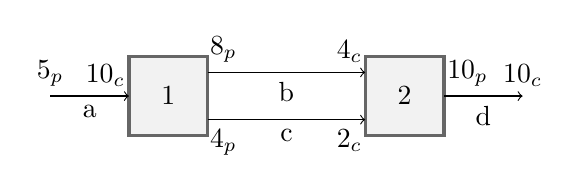
\begin{tikzpicture}[
roundnode/.style={circle, draw=green!60, fill=green!5, very thick, minimum size=7mm},
squarednode/.style={rectangle, draw=black!60, fill=black!5, very thick, minimum size=10mm},
]
%Nodes
\node[squarednode]      (maintopic)   at (5,1)                           {1};
%\node[roundnode]        (uppercircle)       [above=of maintopic] {1};
\node[squarednode]      (rightsquare)      at (8,1) {2};
%\node[roundnode]        (lowercircle)       [below=of maintopic] {4};
 
%Lines
%\draw [help lines] (0,0) grid (10,4);
%\draw[->] (uppercircle.south) -- (maintopic.north);
%\draw[->] (maintopic.east) -- (rightsquare.west);
\draw[->] (3.5,1) -- (4.5,1);
\draw[->] (8.5,1) -- (9.5,1);
\draw[->] (5.5,0.7) -- (7.5,0.7);
\draw[->] (5.5,1.3) -- (7.5,1.3);


\node[align=left, above] at (3.5,1) {$5_p$};
\node[align=left, above] at (5.7,1.3) {$8_p$};
\node[align=left, below] at (5.7,0.7) {$4_p$};
\node[align=left, above] at (8.8,1) {$10_p$};

\node[align=right, above] at (4.2,1) {$10_c$};
\node[align=right, above] at (7.3,1.3) {$4_c$};
\node[align=right, below] at (7.3,0.7) {$2_c$};
\node[align=right, above] at (9.5,1) {$10_c$};

\node[align=left, below] at (4,1) {a};
\node[align=left, below] at (6.5,0.7) {c};
\node[align=left, below] at (6.5,1.3) {b};
\node[align=left, below] at (9,1) {d};

%\draw[->] (rightsquare.south) .. controls +(down:7mm) and +(right:7mm) .. (lowercircle.east);

\end{tikzpicture}
\caption{Do not forget!
Make it explicit enough that readers
can figure out what you are doing.}
\label{fig:example_network}
\end{figure*}

Setting \textbf{U'} as the identity matrix, solving for $a_1$ and $a_2$ results in the linear system:

\begin{equation}
 \begin{cases} 
5=10a_1 \\ 
8a_1=4a_2 \\
4a_1=2a_2 \\
10a_2=10 
\end{cases}
=
 \begin{cases} 
10a_1 = 5 \\ 
8a_1-4a_2=0 \\
4a_1-2a_2=0 \\
10a_2=10 
\end{cases}
\end{equation}

which can be re-written as the augmented matrix:

\begin{equation}
\begin{pmatrix}[cc|c]
  10 & 0 & 5   \\
  8 & -4 & 0  \\
  4 & -2 &  0 \\
  0 & 10 & 10  
 \end{pmatrix}
\end{equation}


Since the rank of the coefficient matrix and the rank of the augmented matrix are both the same, and identical the number of unknowns, this system has unique solution:$a_1=1/2$ and $a2=1$: i.e., actor 1 should run for 50\% of the time. 
\par In this example, there is a solution to the system when \textbf{U'} is the identity matrix; however, this is seldom true. 




